\section{Model Verification}\label{sec:modelVerification}
The parameters used in the final model are taken form previous work on the vessel \cite{thesis}.

\begin{table}[H]
    \begin{tabular}{|c|c|c|}    
        \hline %-----------------------------------------------------------------------------------
        \textbf{Parameter} &\textbf{Value} & \textbf{Units} \\
        \hline %-----------------------------------------------------------------------------------
        $m$  & 13 & kg \\
        $d_{\dot{x}_\mathrm{b}}$  & 2.86 & N$\cdot$m$^{-1}$$\cdot$s \\
        $d_{\dot{y}_\mathrm{b}}$  & 32.5 & N$\cdot$m$^{-1}$$\cdot$s \\
        $I_\mathrm{x}$  & 0.0654 & kg$\cdot$m$^2$ \\
        $I_\mathrm{y}$  & 1.0892 & kg$\cdot$m$^2$ \\
        $I_\mathrm{z}$  & 1.1067 & kg$\cdot$m$^2$ \\
        $d_{\dot{\phi}}$ & 0.1094 &  N$\cdot$m$\cdot$rad$^{-1}$$\cdot$s\\
        $d_{\dot{\theta}}$ & 7.2030 & N$\cdot$m$\cdot$rad$^{-1}$$\cdot$s \\
        $d_{\dot{\psi}}$ & 0.2228 & N$\cdot$m$\cdot$rad$^{-1}$$\cdot$s \\
        $l_1$ & 0.05 & m \\
        $l_2$ & 0.05 & m \\
        $\rho g V \overline{GM_{T}}$ & 6.9736 & N$\cdot$m\\
        $\rho g V \overline{GM_{T}}$ & 131.8316 & N$\cdot$m\\
        \hline %-----------------------------------------------------------------------------------
    \end{tabular}
\end{table}

As it can be seen, the parameters corresponding to the $z_\mathrm{b}$ direction are not presented, since \autoref{eq:z_pos_model_lin} is not used neither for the control design nor for the sensor fusion.

To verify the model a test is carried out. Two constant but different forces are applied to see the turning behavior of the real vessel, as seen in \autoref{app:modelVerification}. The data is then compared to the simulated model when applying the same inputs, and the results can be seen in \autoref{fig:turn} and \ref{fig:turn_time}.

\begin{figure}[H]
    \captionbox 
    {   
        Position of the boat in the $x_\mathrm{n}$-$y_\mathrm{n}$ plane given by the model simulation and the GPS data.
        \label{fig:turn}
    }                                                                 
    {                                                                  
        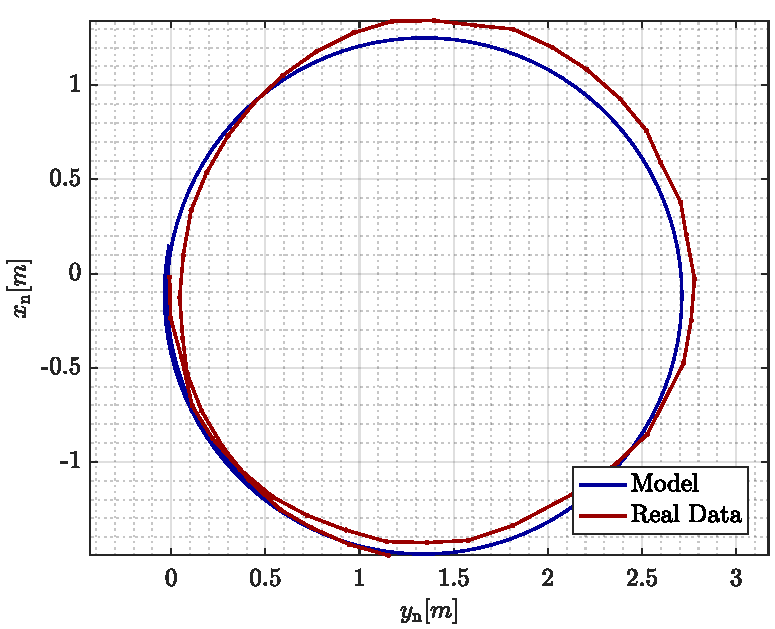
\includegraphics[width=.45\textwidth]{figures/turn}         
    }                                                                    
    \hspace{5pt}                                                          
    \captionbox  
    {      
        $x_\mathrm{n}$ and $y_\mathrm{n}$ with respect to time, both simulated and real.
        \label{fig:turn_time}
    }                                                                        
    {
        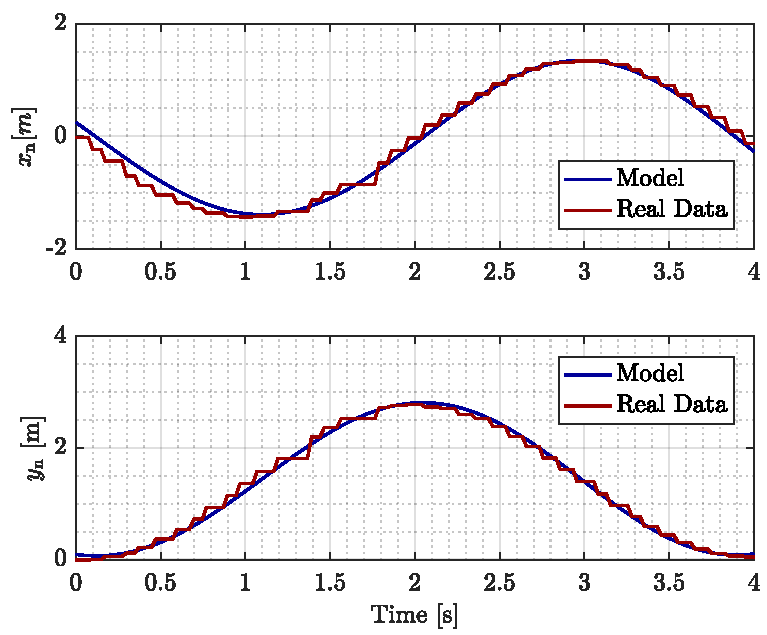
\includegraphics[width=.45\textwidth]{figures/turn_time}
    }
\end{figure}

The results show that the behavior of the real vessel is close to that of the simulated model. It is noticeable that the error between the model and the real behavior is mainly due to the quantization coming from the sampling of the GPS data. Considering this comparison, the model of the vessel is deemed sufficient both for simulation and control design purposes. 

\textit{In this part, the concept and possible applications of ASVs have been introduced with focus on the design of a control system. The possible implications in the design  performing bathymetric measurements have also been considered. In order to characterize the system at hand, the vessel and its components have been described and the vessels behavior has been represented by means of a mathematical model, which constitutes the basis of the control design.}


